
\section{Results}
\label{sec:experiment_results}

	This section provides the results of the experiments listed in Section \ref{sec:experiment_plan}, which are analyzed further in Chapter \ref{ch:analysis}.

\subsection{measuring accuracy}

\begin{table}[H]
	\begin{tabular}{ll}
		\textbf{Adult} & \textbf{Error rate} \\
		Our optimal result (Local model, e=1.0, 10 peer)                  & 0.157 \\
		High privacy, few peers($\epsilon$=0.1, 50 peers)				  & 0.163  \\
		Aggregated model												  & 0.185 \\
		Ensemble model													  &	0.165
	\end{tabular}
	\caption{Measuring accuracy}
	\label{tab:results_measuring_accuracy}
\end{table}

\subsection{Confirming expected effects of differential privacy}
\subsubsection{Changes in $\epsilon$}

\begin{figure}[H]
	\centering
	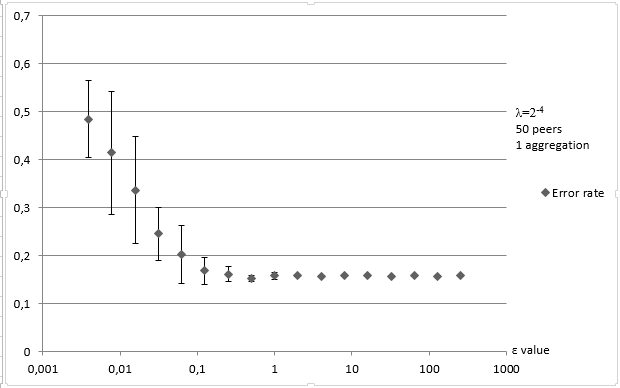
\includegraphics[width=\textwidth]{fig/spambase/epsilon_big_range}
	\caption{Effect of privacy level}
	\label{fig:epsilon_big_range}
\end{figure}

\subsubsection{Changes in $\lambda$}
\begin{figure}[H]
	\centering
	\begin{minipage}{.68\linewidth}
		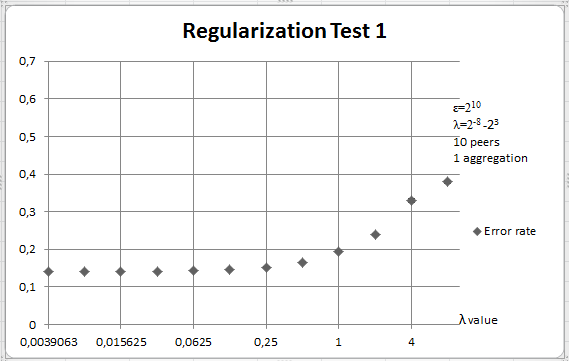
\includegraphics[width=\linewidth]{fig/spambase/regularization_extremelyhighepsilon}
		\captionof{figure}{Effect of regularization, no privacy}
		\label{fig:regularization_extremelyhighepsilon}
	\end{minipage}
	\hspace{1mm}
	\begin{minipage}{.68\linewidth}
		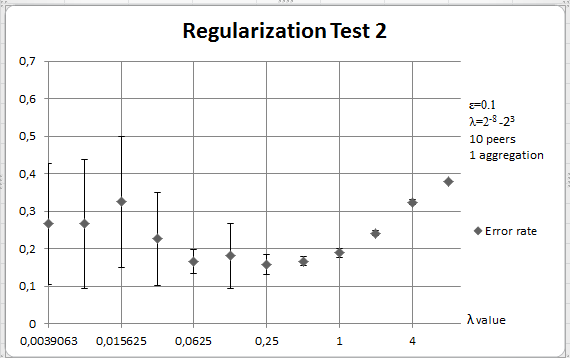
\includegraphics[width=\linewidth]{fig/spambase/regularization_normalepsilon}
		\captionof{figure}{Effect of regularization, common privacy}
		\label{fig:regularization_normalepsilon}
	\end{minipage}
	\hspace{1mm}
	\begin{minipage}{.68\linewidth}
		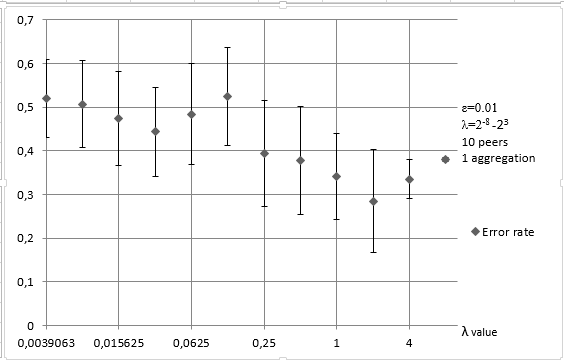
\includegraphics[width=\linewidth]{fig/spambase/regularization_lowepsilon}
		\captionof{figure}{Effect of regularization, high privacy}
		\label{fig:regularization_lowepsilon}
	\end{minipage}
\end{figure}


\subsection{Changes in data availability}
\begin{figure}[H]
	\centering
	\begin{minipage}{.65\linewidth}
		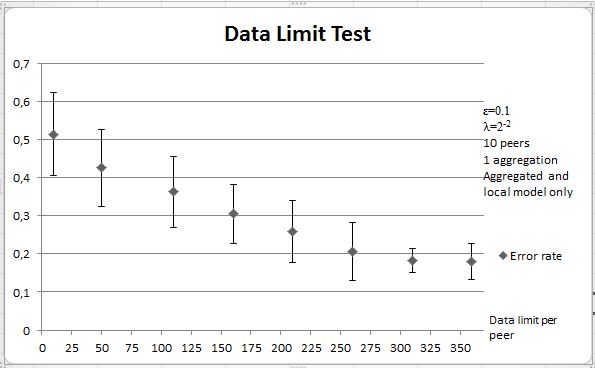
\includegraphics[width=\linewidth]{fig/spambase/data_limit_test_withoutlocalmodel}
		\captionof{figure}{$\epsilon = 0.1, \lambda = 2^{-2}$, 10 peers, 1 aggregations. Aggregated model only.}
		\label{fig:data_limit_test_withoutlocalmodel}
	\end{minipage}
	\hspace{1mm}
	\begin{minipage}{.65\linewidth}
		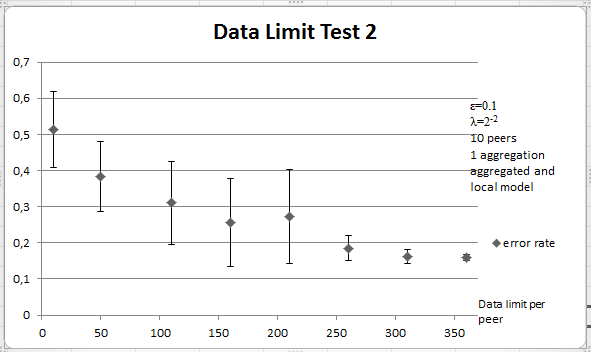
\includegraphics[width=\linewidth]{fig/spambase/data_limit_test_withlocalmodel}
		\captionof{figure}{$\epsilon = 0.1, \lambda = 2^{-2}$, 10 peers, 1 aggregation. Aggregated and local model.}
		\label{fig:data_limit_test_withlocalmodel}
	\end{minipage}
	\hspace{1mm}
	\begin{minipage}{.65\linewidth}
		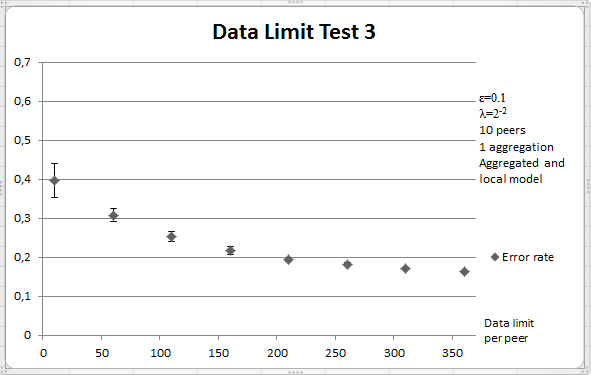
\includegraphics[width=\linewidth]{fig/spambase/data_limit_test_localmodelonly}
		\captionof{figure}{$\lambda = 2^{-2}$, 10 peers, local model only.}
		\label{fig:data_limit_test_localmodelonly}
	\end{minipage}
\end{figure}


\subsection{Changes in number of participants}
%\todo[inline]{make Effect of peer numbers into a simple table row showing min/max instead}
\begin{figure}[H]
	\centering
	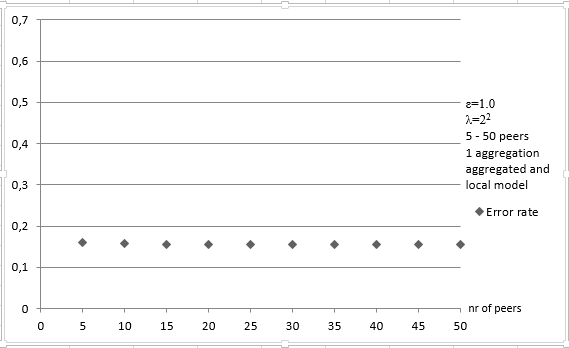
\includegraphics[width=\textwidth]{fig/adult/peer_range_constant_group}
	\caption{Effect of peer numbers.}
	\label{fig:peer_range_constant_group}
\end{figure}


\subsection{Minimizing peer model variance}
%\todo[inline]{replace variance table with numbers from recent, properly CVed runs. ALSO, add std.dev. of std dev. :)}
\begin{table}[H]
	\centering

	\begin{tabular}{|l|l|l|}
		\textbf{Model}                  & \textbf{Mean error} & \textbf{Peer std. dev.} \\
		\hline
		Local, no privacy      & 0,175 & 0.006 \\
		Aggregated, d. privacy & 0,158 & 0.000	 \\
		Ensemble with both & 0.166 & 0.002 \\
	\end{tabular}
	\caption{Variance among peers, Adult}
	\label{table:peer_variance_adult}
\end{table}      

\subsection{Effect of aggregation group sizes}
\begin{figure}[H]
	\centering
	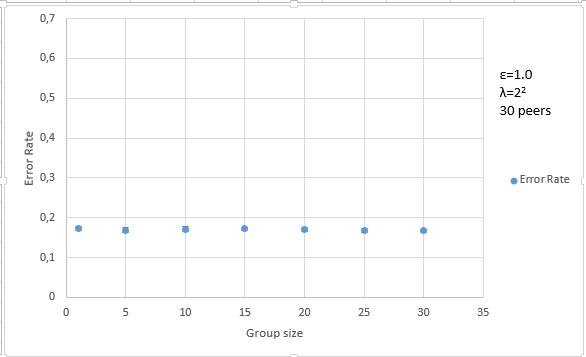
\includegraphics[width=0.8\textwidth]{fig/adult/GroupSizeTest}
	\caption{Effect of Aggregation Group Sizes.}
	\label{fig:results_group_sizes}
\end{figure}

%add - some result comparing difference between party and all publishing



\subsection{Value of budgeting privacy}

\begin{figure}[H]
	\centering
	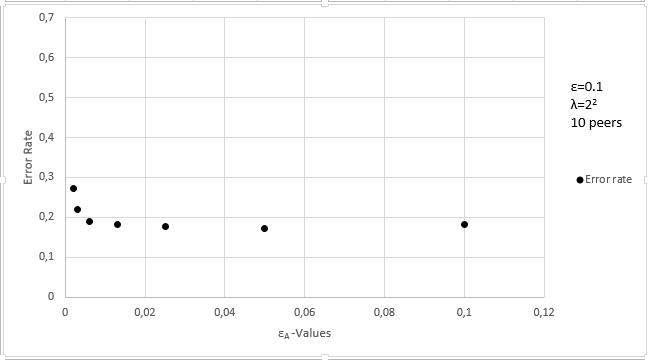
\includegraphics[width=.8\textwidth]{fig/adult/results_privacy_budget}
	\caption{Effect of Privacy Budgeting.}
	\label{fig:results_privacy_budget}
\end{figure}


%add - some result showing what happens when the amount of privacy budget used is changed - possibly considering all vs party also here


\cleardoublepage